\section{Bulletin D'Expedition}

\begin{figure}[htbp]
\centering
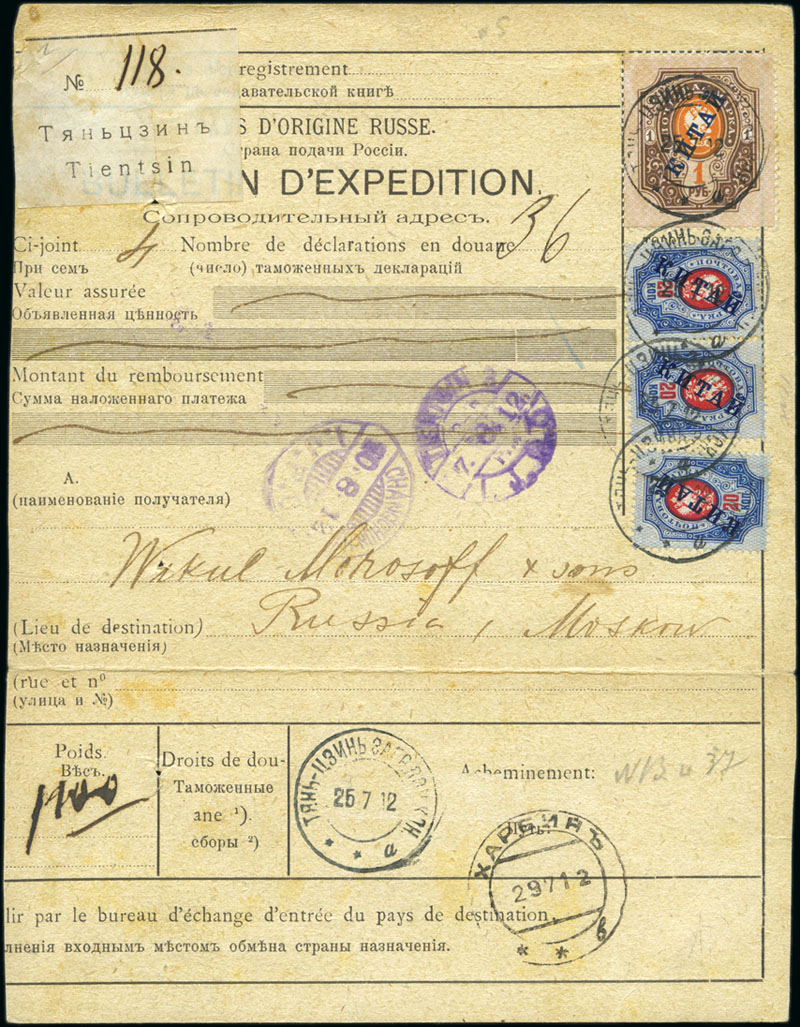
\includegraphics[width=.95\textwidth]{../russian-post-offices-in-china/10011.jpg}
\caption{
10011 TIENTSIN: 1912 Dispatch document (Bulletin D'Expedition) for consignment to
Moscow without declared value, franked with "KITAI" 1R and three 20k tied by 
Tientsin 25.7.12 cds (T\&S type 5C), with white bilingual registration label 
at top left, with transit datestamp of the Japanese P.O.s at Tientsin and Changchun, 
the Russian P.O. at Harbin (Manchuria) and Moscow, rare and unusual.
Note: The Harbin ds is an unrecorded subtype
\euro 400.00
}  
\end{figure}

\begin{figure}[htbp]
\centering
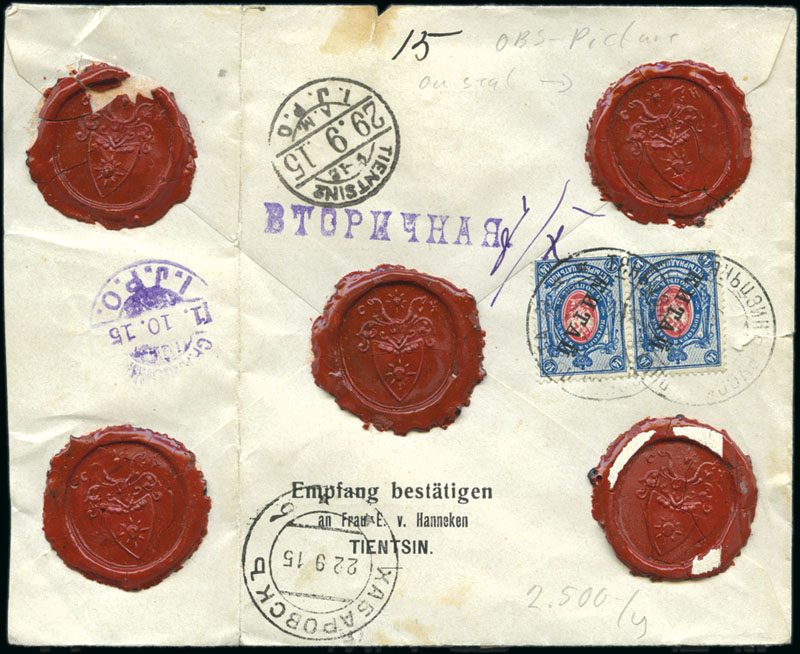
\includegraphics[width=.95\textwidth]{../russian-post-offices-in-china/10012.jpg}
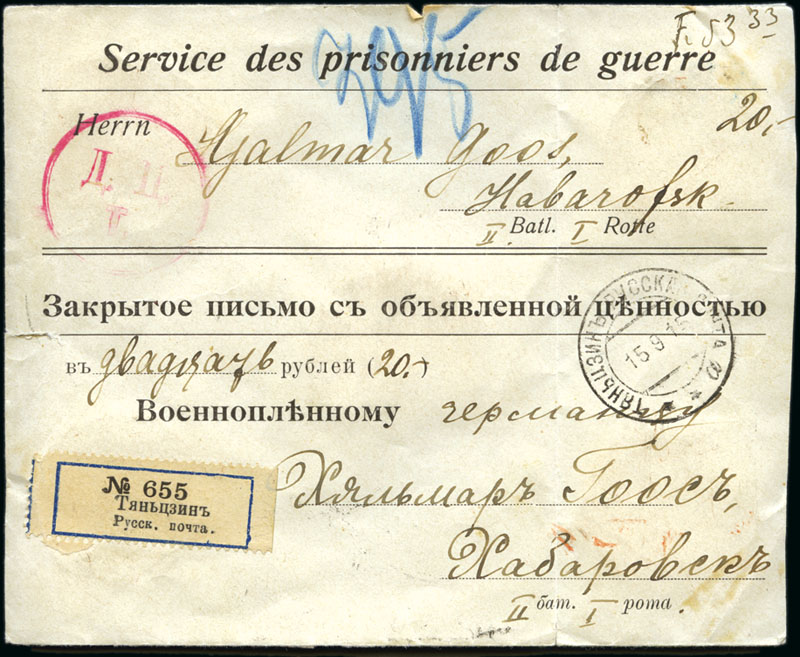
\includegraphics[width=.95\textwidth]{../russian-post-offices-in-china/10012-1.jpg}
\caption{
10012	TIENTSIN: 1915 Prisoner of War printed envelope sent insured for 20R to P.O.W.
at Khabarovsk (Siberia), franked on the reverse with "KITAI" 14k pair tied by
Tientsin 15.9.15 cds (Tchilinghirian type 6), sent via the Japanese P.O.s at 
Tientsin and Changchun, with insured label in Cyrillic on obverse, with 
Pogranichnaya censor hs, s/l Vtorichnaya hs indicating 2nd delivery attempt
and five attractive wax seals.
\euro 400.00
}  
\end{figure}

\begin{figure}[htbp]
\centering
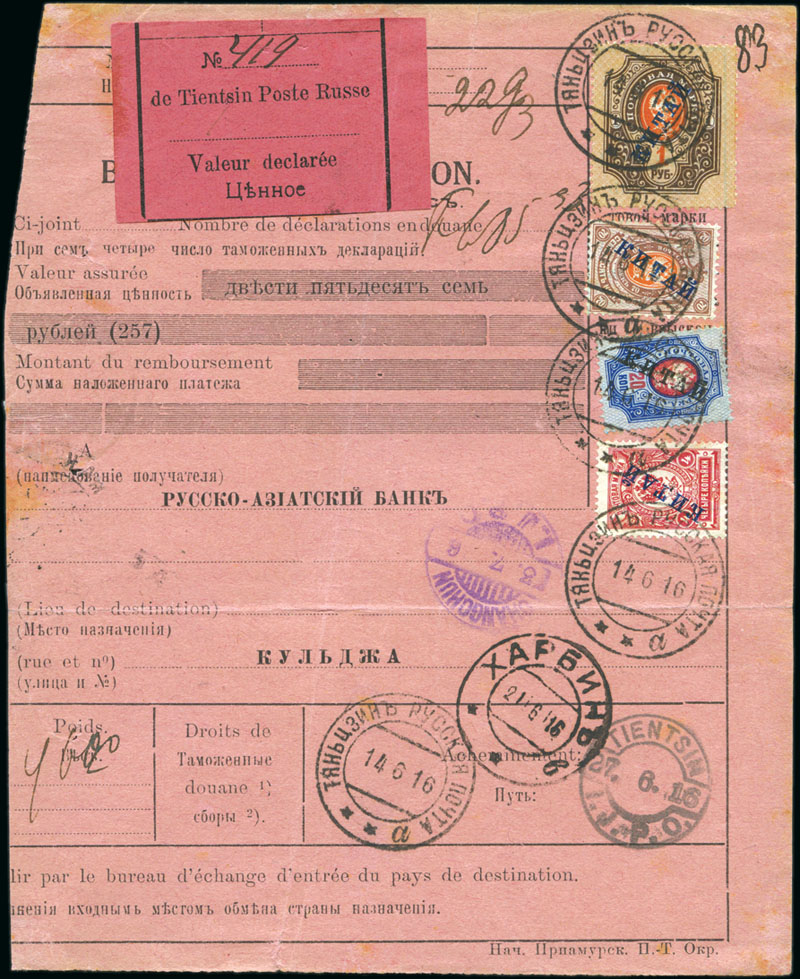
\includegraphics[width=.95\textwidth]{../russian-post-offices-in-china/10013.jpg}
\caption{
10013 TIENTSIN: 1916 Despatch card ( du destinataire) for value declared 
packet to Kuldja (SINKIANG), franked with "KITAI" 4k, 20k, 70k and 1R tied by 
Tientsin 14.6.16 cds (T\&S type 6), with red "valeur declar\'ee" label adjacent, s
ent via the Japanese P.O.s at Tientsin and Changchun and the Russian P.O. at 
Harbin, arriving in Kuldja 20.7.16 (error "19" for "16"), the International 
card was used because the postal route to Sinkiang took the packet outside 
China, re-entering via the Russian province of Semirechinksk
Currently \euro 800.00
}  
\end{figure}

\begin{figure}[htbp]
\centering
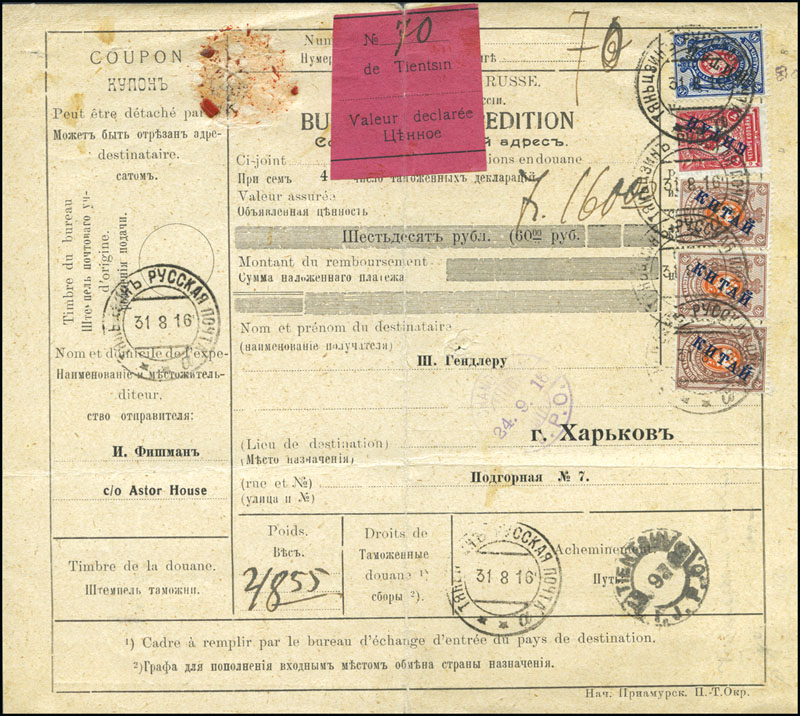
\includegraphics[width=.95\textwidth]{../russian-post-offices-in-china/10014.jpg}
\caption{
10014 TIENTSIN: 1918 Dispatch document (complete) for sending valued at 60R to 
Kharkov, franked with "KITAI" 4k, 14k and 70k (3) tied by Tientsin 31.8.16 cds 
(T\&S type 6), red value declared (valeur declar\'e) label, sent via the 
Japanese P.O. at Changchun, rare as normally the left 
hand side "Coupon" was detached on arrival.
\euro 700.00 
}  
\end{figure}

\begin{figure}[htbp]
\centering
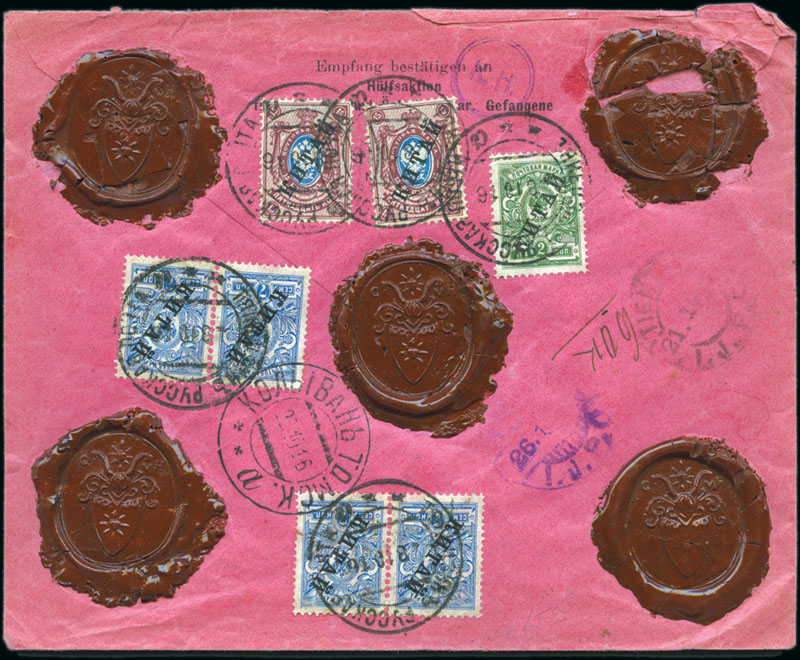
\includegraphics[width=.95\textwidth]{../russian-post-offices-in-china/10015.jpg}
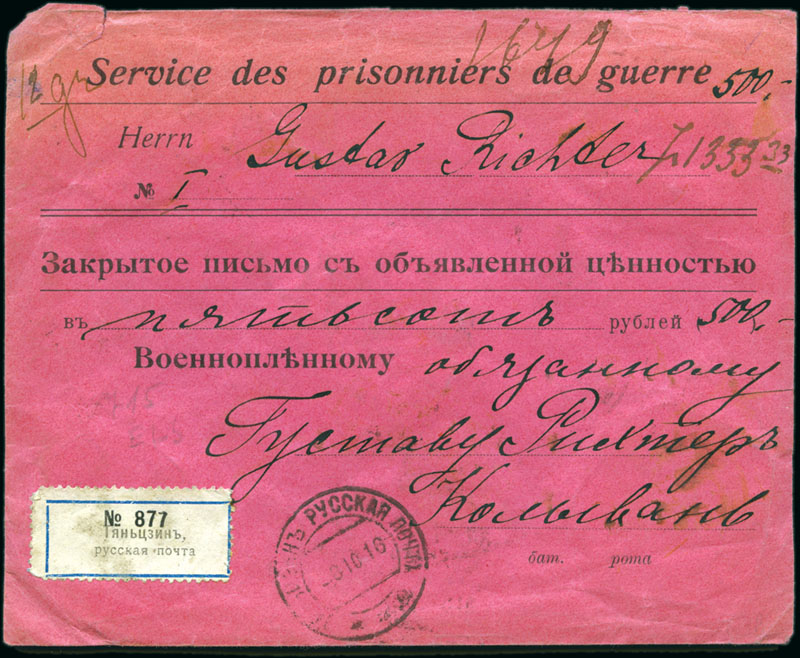
\includegraphics[width=.95\textwidth]{../russian-post-offices-in-china/10015-1.jpg}
\caption{
10015	TIENTSIN: 1916 Prisoner of War printed envelope sent insured for 500R
to P.O.W. at Kolyvan (Siberia), franked on the reverse with "KITAI" 2k, 7k (2 pairs)
and 15k (2) all tied by Tientsin 8.10.16 cds (T\&S type 6), sent via the 
Japanese P.O.s at Tientsin and Changchun, with insured label on obverse, 
wax seals on reverse, attractive.
\euro 300.00
}  
\end{figure}








                                                        